% Fig 3.6 — BM25 query repetition mechanism (from Query2Doc paper)
\documentclass[border=4pt]{standalone}
\usepackage{tikz}
\usetikzlibrary{positioning, arrows.meta}
\begin{document}
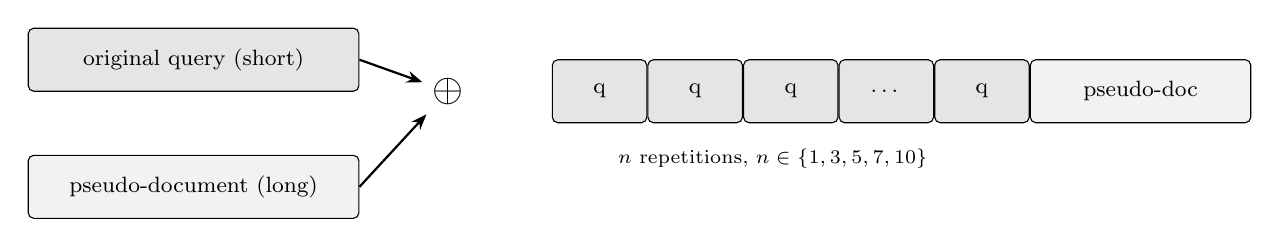
\begin{tikzpicture}[
    >=Stealth, node distance=8mm and 14mm,
    box/.style={rectangle, draw, rounded corners=2pt,
                minimum height=8mm, align=center, font=\footnotesize},
    arrow/.style={-{Stealth[length=2mm]}, thick}
]
  % left: short user query
  \node[box, fill=black!10, minimum width=42mm] (q) {original query (short)};
  \node[box, fill=black!5, below=of q, minimum width=42mm] (pd) {pseudo-document (long)};

  % middle: concatenation operator
  \node[right=of q, xshift=-6mm, yshift=-4mm, font=\Large] (op) {$\oplus$};

  % right: repeated query concatenation
  \node[right=of op, xshift=-4mm, box, fill=black!10, minimum width=12mm] (qa) {q};
  \node[right=0mm of qa, box, fill=black!10, minimum width=12mm] (qb) {q};
  \node[right=0mm of qb, box, fill=black!10, minimum width=12mm] (qc) {q};
  \node[right=0mm of qc, box, fill=black!10, minimum width=12mm] (qd) {\dots};
  \node[right=0mm of qd, box, fill=black!10, minimum width=12mm] (qn) {q};
  \node[right=0mm of qn, box, fill=black!5, minimum width=28mm] (pdr) {pseudo-doc};

  \node[below=2mm of qa, font=\scriptsize, xshift=22mm] {$n$ repetitions, $n \in \{1,3,5,7,10\}$};

  \draw[arrow] (q.east) -- (op);
  \draw[arrow] (pd.east) -- (op);
\end{tikzpicture}
\end{document}
